\documentclass[tikz,border=3pt]{standalone}
\usepackage[utf8]{inputenc}
\usepackage[T1]{fontenc}
\usepackage{lmodern}
\renewcommand{\familydefault}{\sfdefault}
\usepackage{sansmath}\sansmath
\usepackage{chemfig}
\usepackage{pgfplots}\pgfplotsset{compat=1.18,/pgf/number format/use comma,/pgf/number format/1000 sep={.}}
\usetikzlibrary{arrows.meta,calc,positioning,decorations.pathmorphing,patterns}
% paleta del sitio
\definecolor{nar}{HTML}{E8680C}\definecolor{narc}{HTML}{FFB35C}\definecolor{hielo}{HTML}{FFF3E8}
\definecolor{tinta}{HTML}{1D1D1F}\definecolor{gris}{HTML}{6E6E73}\definecolor{lila}{HTML}{7C5CF0}
\definecolor{azul}{HTML}{2F6FD6}\definecolor{menta}{HTML}{17A673}\definecolor{coral}{HTML}{E8342A}
\begin{document}
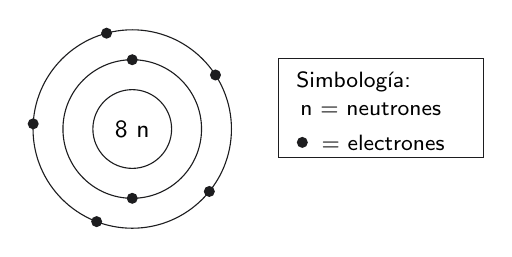
\begin{tikzpicture}[font=\small]
\draw[tinta] (0,0) circle (0.88);
\fill[tinta] (0,0.88) circle (0.07);
\fill[tinta] (0,-0.88) circle (0.07);
\draw[tinta] (0,0) circle (1.26);
\fill[tinta] (-0.326,1.217) circle (0.07);
\fill[tinta] (1.057,0.686) circle (0.07);
\fill[tinta] (0.979,-0.793) circle (0.07);
\fill[tinta] (-0.452,-1.176) circle (0.07);
\fill[tinta] (-1.258,0.066) circle (0.07);
\draw[tinta,fill=white] (0,0) circle (0.5);
\node[align=center,font=\small,inner sep=0] at (0,0) {8 n};
\draw[tinta] (1.86,0.9) rectangle (4.46,-0.36);
\node[anchor=north west,font=\footnotesize] at (1.96,0.85) {Simbología:};
\node[anchor=west,font=\footnotesize] at (2.01,0.25) {n = neutrones};
\fill[tinta] (2.16,-0.17) circle (0.07);
\node[anchor=west,font=\footnotesize] at (2.28,-0.17) {= electrones};

\end{tikzpicture}
\end{document}
